\chapter{Analysis}
\section{Introduction} \label{introduction}
The goal of this project is to build a new system for a teacher who runs a chess club at Alleyn's School, London. In this section, research has been done to learn what the current system does. This research will inform me of what the new system that I will build should be able to do and what additional features it will provide over the current implementation. My research consisted of giving a questionnaire to the user and of researching the rules of chess.
\section{Rules of Chess}
As with any game, there are rules that have to be adhered to for a valid game to be played. For me to have a viable solution to the problem identified, the program I create must follow the rules of chess. Thus in this section I will discuss what these rules are.
\subsection{The Game Board}
\begin{figure}[H]
\centering
	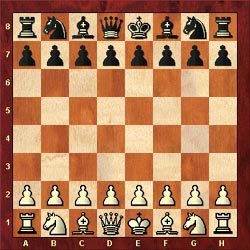
\includegraphics[width=0.3\textwidth]{images/boards/initial_board}
	\caption{The initial setup of a game of chess.}
	\label{initial-board}
\end{figure}
The initial starting position of the board contains all the types of pieces in the game: pawn, king, queen, bishop, knight and rook. From this point onwards, white is the first to move. Once white has completed a legal move it is then black's turn to do the same and the game continues until the game has reached the state of checkmate or stalemate, which will be explained in detail later. Only one piece can occupy a square on the board, thus a piece cannot take one of its own pieces but can capture opposing pieces as long as it isn't a king.

\paragraph{Note:}when the types of moves that a certain type of piece can make are discussed below, it is assumed that when moved, it does not put the player who is moving the piece into check. In addition, it will be assumed that the move does not mean that the moving piece is in the same place. If this is the case then the move is illegal.
\subsection{Pawns}
\begin{figure}[H]
\centering
	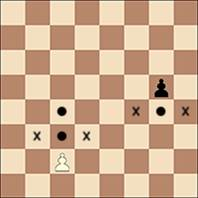
\includegraphics[width=0.3\textwidth]{images/boards/pawn_movement}
	\caption{The possible moves a pawn can make.}
\end{figure}
The pawn is a type of piece and has two types of moves, depending on the situation. If the pawn is in the same space as its starting position then it can either move one or two spaces forward, given that there is no piece in the way of this movement. In any other position it is only able to move into the next square forward, as long as there is no other piece currently there. It is also able to capture any opposing pieces that are diagonally in front of it.
\subsubsection{Promotion}
\begin{figure}[H]
\centering
	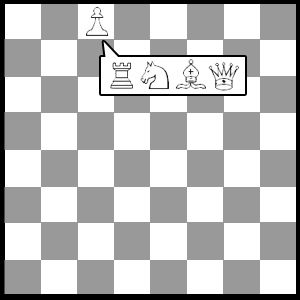
\includegraphics[width=0.3\textwidth]{images/boards/promotion}
	\caption{The types of pieces that a pawn can be promoted to.}
\end{figure}
When a pawn reaches the other side of the board the pawn must be changed to an additional piece that is a rook, knight, bishop or queen.
\subsubsection{En Passant}
\begin{figure}[H]
\centering
	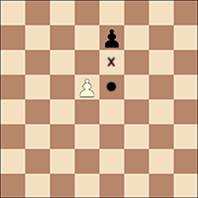
\includegraphics[width=0.3\textwidth]{images/boards/en_passant}
	\caption{A board position in which en passant is possible.}
\end{figure}
As can be seen above, if a pawn is moved two spaces forward such that it is horizontally adjacent to an opposing pawn once it is moved, the opposing pawn has an opportunity to capture the pawn and move to the 'x' marked on the diagram. When this opportunity occurs, whether it is taken or not, it cannot be done again by that player for the rest of the game.
\subsection{Kings}
\begin{figure}[H]
\centering
	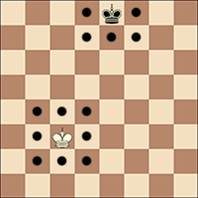
\includegraphics[width=0.3\textwidth]{images/boards/king_movement}
	\caption{The possible moves of a king.}
\end{figure}
The king can move to any adjacent square provided that it is not in check once it completes the move. In addition it should not be adjacent diagonally, horizontally or vertically, to the opposing king after it has moved. 
\subsubsection{Castling}
\begin{figure}[H]
\centering
	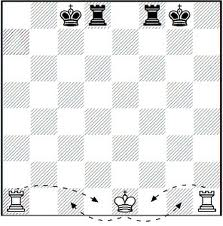
\includegraphics[width=0.3\textwidth]{images/boards/castling}
	\caption{Movement of king and rook during castling.}
\end{figure}
Castling is a move (shown above) that can be performed only if the king and rook have not been moved before. For castling to be performed no pieces must be in the way of the king and the rook moving and any of the squares in between them must not be attacked by an opposing piece. The king cannot castle when it is under attack.
\subsection{Bishop}
\begin{figure}[H]
\centering
	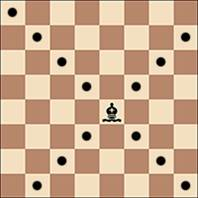
\includegraphics[width=0.3\textwidth]{images/boards/bishop_movement}
	\caption{The possible moves of a bishop.}
\end{figure}
The bishop can move diagonally in any direction. Thus, it can only move on the colour of squares that are the same as its starting position.	
\subsection{Rook}
\begin{figure}[H]
\centering
	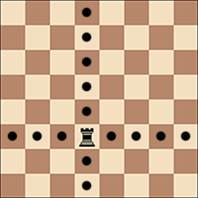
\includegraphics[width=0.3\textwidth]{images/boards/rook_movement}
	\caption{The possibles moves of a rook.}
\end{figure}
The rook can move both vertically and horizontally in any direction.
\subsection{Queen}
\begin{figure}[H]
\centering
	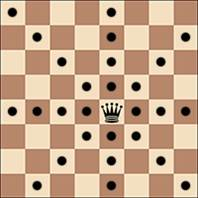
\includegraphics[width=0.3\textwidth]{images/boards/queen_movement}
	\caption{The possible moves of a queen.}
\end{figure}
The queen can both move anywhere diagonally, horizontally and vertically. In other words, a queen can be considered a combination of both the rook and the bishop.
\subsection{Knight}
\begin{figure}[H]
\centering
	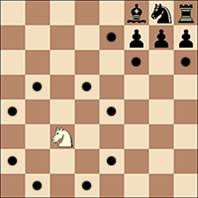
\includegraphics[width=0.3\textwidth]{images/boards/knight_movement}
	\caption{The possible moves of a knight.}
\end{figure}
The knight has one of the more interesting moving patterns. It can move in what is known as an L-shape. To be more precise, the possible moves of a knight can be calculated by moving 2 along vertically and then 1 horizontally either side, and vice-versa. Its attacking moves do not include the path to its possible moves.
\subsection{Game States}
In chess there are 3 types of game states that differ from normal play and restrict what legal moves can be made. Two of those are permanent (end of game) states: checkmate and stalemate. The other is check and this means that only moves that take a player out of check can be made. 
\subsubsection{Check}
\begin{figure}[H]
\centering
	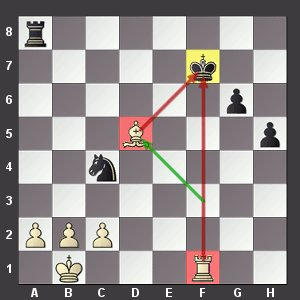
\includegraphics[width=0.3\textwidth]{images/boards/check_example}
	\caption{An example of check.}
\end{figure}
Check occurs when a piece moves such that it is attacking the opposing king. An attacking move is such that if we theoretically suppose that the king is a piece that can be captured by a piece, then it would be captured if the piece moved there. An example of this is the image seen above. An important note is that for pawns this means they cannot check a king if it is horizontally ahead of it, as a pawn cannot move there if we theoretically supposed that a king is able to be captured. However, it can if the king is diagonally adjacent in front of the pawn. 
\subsubsection{Checkmate}
\begin{figure}[H]
\centering
	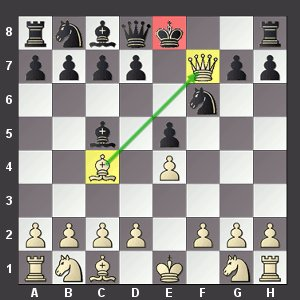
\includegraphics[width=0.3\textwidth]{images/boards/checkmate_example}
	\caption{An example of checkmate.}
\end{figure}
Checkmate occurs when a player is put into check and cannot make a move that brings themselves out of check. The person who is in check is the loser of the game and thus the opposing player is the winner. A well-known example is the scholar's mate which can be seen above. The queen cannot be taken by any piece and the king has nowhere to move without still being in check. In addition, the king cannot take the queen as it will put itself in check to the bishop. Thus black concedes the game as it is in a state of checkmate.
\subsubsection{Stalemate}
\begin{figure}[H]
\centering
	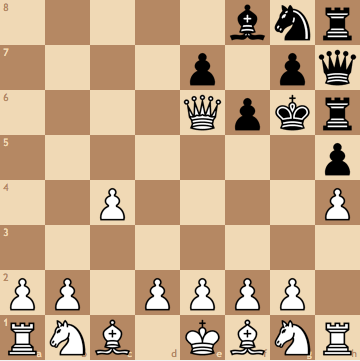
\includegraphics[width=0.3\textwidth]{images/boards/stalemate_example}
	\caption{An example of stalemate.}
\end{figure}
Stalemate occurs when a player who is not in check cannot make any legal moves and thus the game cannot continue. Above is an example of a stalemate. It is black's turn to move but it has no legal moves to make. Any movements are either not available to make or expose the king to being in check to either the far-right pawn or the queen. When a stalemate occurs the game is declared as drawn and there are no winners or losers.
\section{Questionnaire}
As mentioned in section~\ref{introduction}, a questionnaire would form part of my research. The teacher who runs the chess club is the one who has answered the following questionnaire. In this questionnaire, it is determined what the current system does, the problems it has, and the objectives of the new system which I will be creating.

\textbf{Explain the background of the current system.}

I work at Alleyn's School in Dulwich as a teacher and run the chess club every Wednesday lunch. Pupils from ages 11-18 are allowed to play chess. Every year we run an inter-house chess competition, where each house of the school assembles a team together to determine which house is best at chess. Approximately 20 pupils show up to the club every week, with this number rising to about 50 during competitions. The inter-house chess competition is particularly popular and I run it once a year for about 4 or 5 weeks. The competition take place in two rooms in the Science Department. The competition is played on approximately 25 Chess Boards.  

\textbf{What kind of data is stored on the system and how is it processed?}

When the chess competition happens, we must store data on the results of individual games. Specifically, we store the names of the player and the winner of each game. The game board used by the players serves as a way of recording the state of the game. The game board also serves as a way of making moves and seeing moves being made. The rules of the game are adhered to by the players themselves, as it is assumed that is in the best interest of each player to make sure that the other is not cheating. If a game overruns past lunchtime, then the players can take a picture of the board and then continue the game later. This information is currently displayed on the whiteboard during the lunchtime of the competition, and then is transferred to my personal notebook once lunchtime is over. 

\textbf{What problems does this current system have?}

Firstly, there can be times where there are disagreements between two players over the game. The issues tend to be centred around possible cheating. It would be good to have a system where arguments over cheating would not occur. Secondly, there are many clubs and activities run at the school, which clash with chess club. This results in people who cannot play chess with us even though they want to. It would be nice to be able to allow people to play chess outside of school hours. Thirdly, whilst a photo of the game board can be taken to allow the game to be continued elsewhere if it runs over lunch, information about whether en passant is still possible and who’s move it is cannot be saved via a picture.  In addition, when a chess competition occurs, many players are interested in seeing the results of certain games. However, as all games are stored on my notebook students are usually individually told or e-mailed the results of games if they are interested. It would be useful to have a system in place where interested parties can view the results of all chess games played in their own time.

\textbf{What data would you like to be stored in a new system?}

I would like for games to be stored. The data on each game should be such that it is possible to continue playing later. Thus, it must include the position of all the pieces on the board, the current game state (e.g. is a player in check?), whether en passant is possible and where it can occur, and whose turn it is. In addition, the names of both players must be stored, the number of moves made, when the last time the game was played and the name of the winner if there is one. 

\textbf{Could you outline the core requirements of the new system?}

The new system should be able to identify all the legal moves of a given piece and display this information clearly to the user. In addition, the game must be able to identify changes in the state of the game and display these changes to the user when they occur. These requirements must be satisfied as it should be possible to play chess using this new system, where moves can be made and the results of these moves should be clearly shown. All games that are played must have the ability to be saved, including the names of the players, so that the game can be played at a later date. Thus, all games that are saved must be able to be easily loaded by the user.
\section{Setting}
The program was designed for the school's Chess club and is open for students from year 7 to 13. Chess club currently runs weekly at lunchtimes and is run by a physics teacher – Dr De Silva. Every year a primarily student run inter-house chess competition, with each house having a team of avid chess players, takes place to determine which house has the best chess players. As a member of chess club I identified and researched problems with the current system that the club uses. I also consulted with Dr De Silva about any problems that he has noted in the current system and have used this information to aid me in determining the objectives that I plan for the new system to implement.
\section{Users}
The primary users are those students who partake in the chess club and actively play chess amongst one another. It can also be used by the teacher that runs the club to record the results of games, which is paramount when there are competitions taking place. There is an additional benefit in that it can be played at any time and on any computer in the school area that has the program installed. This may be of good use to those who would like to play chess but are unable to go to the club due to other extra-curricular activities.
\section{System}
Currently most games that are played are not recorded because most are for recreational entertainment and so the result of the game is inconsequential, though results may be remembered by students and also may help in choosing players for the inter-house chess competition. Currently, when the inter-house chess competition happens the whiteboard in the classroom is used to show players who they are playing against and when the game is finished the result is written to the right of the matchings. Then the results are transferred to paper and are stored by the teacher who runs the club.
\section{Input}
All the results of games to do with a competition are recorded in a notebook and of course the movement of pieces is recorded on the board. All other games are not recorded at all and the location of pieces when a game is finished are generally not stored unless a student chooses to take a picture of the board.
\section{Processing}
Processing in the current system is fairly simple. Once a player has chosen where to move a piece, they pick it up and move it to the appropriate position on the board. If it is illegal it is assumed that the opponent will notice as it is in their best interest to not allow such a move. If that is the case then the piece is simply moved back to its place. The player who moves a piece also notes mentally if the piece that they have moved has resulted in a change in the state of the game.
\section{Output}
Output is simply where the player moves their piece on the board, which is visible to both players and any people watching. In addition, when a player moves a piece which results in the changing of the game state they must state this change openly to the opposing player.
\section{Volumetrics}
In this particular application it is hard to estimate the memory needed to store the data needed to play a game as the data required is dynamic. However, we can make some assumptions about the game and use this to estimate the memory required. 

Firstly, I'll discuss the byte allocations that the Python programming language gives to certain objects and data structures:
\begin{table}[H]
\centering
	\begin{tabular}{| l | l | l |}
		\hline
		\textbf{Bytes} & \textbf{Type} & \textbf{Details} \\ \hline
		24 & int & \\ \hline
		24 & bool & an instance of an int\\ \hline
		52 & str (unicode) & +4 byte per additional character. \\ \hline
		72 & list & +32 for first element, 8 thereafter. \\ \hline
		280 & dict & 6th item increases to 1048; 22nd, 3352; 86th, 12568 * \\ \hline
	\end{tabular}
	\caption{Byte allocations for primitive data types in Python.}
\end{table}
Firstly, the game is stored in a 2D $ (8\times8) $ list object, with each element of the list containing either an integer with value 0 or a Piece object. However, this is not how the data is stored in the JSON file. Instead, the JSON file mimics all the attributes of the \mintinline{python}/class Board(object)/, apart from the \mintinline{python}/board/ attribute.

In the following table, a list of all the attributes of the board class are contained with the type that they will be stored as in the JSON file. This table will show how many bytes are required to store a game as an upper bound. It is assumed that the player names are 10 characters long, which is unlikely to be the case for one player, let alone two. In addition, it is assumed that no pieces are taken, as if that is the case, then the size of the file will inevitably be smaller.

\begin{table}[H]
	\resizebox{\textwidth}{!}{%
	\begin{tabular}{| l | l | l | l |}
		\hline
		\textbf{Attribute} & \textbf{Type} & \textbf{Bytes} & \textbf{Occurence}\\ \hline
		id & int & 24 & 1\\ \hline
		player{\_}one & str  & $ 52+4\times8=84 $ (assuming 10 characters).& 1\\ \hline
		player{\_}two & str  & $ 52+4\times8=84 $ (assuming 10 characters).& 1\\ \hline
		last{\_}played & str & $ 52+4\times10=92 $ (in format dd/mm/yyyy) & 1\\ \hline
		turn & str & $ 52+4\times5=72 $ ("White" or "Black")& 1\\ \hline
		move{\_}num & int & 24 & 1\\ \hline
		winner & str & $ 52+4\times5=72 $ ("White" or "Black")& 1\\ \hline
		colour{\_}in{\_}check & str & $ 52+4\times5=72 $ ("White" or "Black")& 1\\ \hline
		is{\_}stalemate & bool(int) & 24 & 1\\ \hline
		game{\_}over & bool(int) & 24 & 1\\ \hline
		must{\_}promote & bool(int) & 24 & 1\\ \hline
		enpassant{\_}possible & dict & 280 & 1\\ \hline
		enpassant{\_}possible['Black'] & bool(int) & 24 & 1\\ \hline
		enpassant{\_}possible['White'] & bool(int) & 24 & 1\\ \hline
		enpassant{\_}move & dict & 280 & 1\\ \hline
		enpassant{\_}move['from'] & list & $ 72+32+24+8+2=150 $ & 1\\ \hline
		enpassant{\_}move['to'] & list & $ 72+32+24+8+24=150 $ & 1\\ \hline
		enpassant{\_}move['taken'] & list & $ 72+32+24+8+24=150 $ & 1\\ \hline
		pieces & dict & 280 & 1\\ \hline
		pieces[*] & dict & 280 & 5\\ \hline
		pieces[*]['position'] & list & $ 72+32+24+8+24=150 $ & 32 (all pieces)\\ \hline
		pieces[*]['colour'] & str & $ 52+4\times5=72 $ ("White" or "Black")& 32 (all pieces)\\ \hline
		pieces[*]['first{\_}moved'] & int & 24 & 16 (all pawns)\\ \hline
		pieces[*]['has{\_}moved'] & list & $ 72+32+24+8+24=150 $ & 6 (rooks and kings)\\ \hline
		\multicolumn{2}{|r|}{\textbf{Total}} & \multicolumn{2}{|l|}{11,722 bytes} \\ \hline
	\end{tabular}}
	\caption{Bytes required for the storing of one chess game.}
\end{table}
Whilst the following table helps to calculate the size of storing each game, it is not taken into account the overhead of the game list. Thus the formula, $ f(x) $, where $ x $ is the number of games stored, for the upper bound in bytes of the JSON file is:\[ f(x) = (11722)x + (72+32) + 8(x-1) = 11730x + 96\]
\section{Problems with the Current System}
The current system consists of chess boards with pieces and paper if results want to be recorded. The main problem that was noticed was that as the club was only hosted on a single lunchtime a week, many games overran past lunchtime and so had to be stopped with no clear winner as the game had not finished. As the game was played on a physical board with pieces and the room that was used for the club is used for lessons as well, the current state of the game is not saved which resulted in the game effectively being cut short. This is incredibly frustrating, especially for higher-level players as their games tend to take longer to finish. 

Another problem came from when in-school chess competitions occurred. These competitions required results to be recorded such that it could be determined who plays who in further rounds of the competition, i.e. what teams play against one another in the final. These are recorded at lunchtime on the board and then recorded later on paper. There are of course problems with such a system. Firstly, results can easily be lost as it is held in one location. This also means that only one person can view the results at the time, unless the results are published in an e-mail which takes time to produce. In addition, it does not store the final state of the game when finished which may be of interest to students and teachers alike.

A problem that has been noted by students is that even though they are willing to attend chess club, many are unable to attend at lunchtimes on a certain day because they have other commitments and so end up not attending at all despite their desire to do so. Many students would like to be able to play chess games outside of club hours amongst each other with results recorded at school.
\section{Objectives} \label{objectives}
After the analysis of the current system and the requirements that would be needed for an improved system I have created SMART (Specific, Measurable, Achievable, Realistic and Timely) objectives which make clear to me - the developer – what the client requires for their new system which has been determined to be feasible to complete and adheres to all of the letters of the SMART abbreviation.

The objectives of the new system are as follows:
\begin{enumerate}
	\item The showing of an interactive chess board allowing movement of pieces by users which adheres to all chess rules.
	\begin{enumerate}
		\item When program loads, show default chess starting position (a new game).
		\item Ensure only pieces of the moving player's corresponding colour are clickable.
		\item When a piece is clicked calculate all of its legal moves.
		\begin{enumerate}
			\item For each type of piece calculate where it could possibly go assuming there are no other pieces on the board (i.e. bishops diagonally, rooks horizontally/vertically etc.).
			\item Taking into account where other pieces are on the board, calculate the possible moves for that piece.
			\item If we are checking moves for a king, check that castling is possible. If we are checking moves for a pawn, check that en passant is possible.
			\item Considering the moves that have been calculated, check that each position does not result in the moving player to be in check. 
			\begin{enumerate}
				\item If a move results in a player going into check then remove that move from the list of legal moves.
			\end{enumerate}
			\item When this calculation is done, cells in the table corresponding to the legal moves must be made clickable so that the player can move the appropriate piece there if they wish.
			
		\end{enumerate}
		\item After a piece is moved perform a check of the game state. If the state has changed (i.e. if a player has been put into check or the game has ended) then inform the user of this via a dialog.
		\item If the pawn has successfully reached the other side of the board, then open a dialog to let the user decide to what piece the pawn should be converted to.
	\end{enumerate}
	\item Allow the editing of player's names via textboxes.
	\item Allow a game that is currently in play to be saved.
	\begin{enumerate}
		\item If there is no file path to save the game to, prompt the user for a path and filename to save a new JSON file to.
		\item If there is a file path and the JSON file is found, then save the game to the file.
		\item If there is a file path and the JSON isn't found, then prompt the user for a path and filename to save a new JSON file to.
		\item If a game has been successfully saved, convey this information to the user via a dialog.
		\item If the player names have not been filled in, then do not save the game and inform the user that they have to fill in the names in the form of a dialog.
		\item If the game has an ID then save it by replacing the element of the games array with the same name by searching for the appropriate ID with a binary search.
	\end{enumerate}
	\item Allow a user to load a game and to continue to play it.
	\begin{enumerate}
		\item If the JSON file is not found then prompt the user to input the path to the game.
		\item Display the list of games in a table to allow the user to know which game to choose.
		\begin{enumerate}
			\item Information that must be shown in the table: ID, name of player 1 and 2, winner, moves made, last played.
			\item Using a quicksort algorithm, allow the user to sort the list of games based on parameters such as ID and the names of players.
		\end{enumerate}
	\end{enumerate}
\end{enumerate}